
\documentclass{beamer}
\usecolortheme{dove}
\setbeamertemplate{navigation symbols}{}
\usepackage{amsmath,amssymb,amsfonts,amsthm, multicol, subfigure, color}
\usepackage{bm}
\usepackage{graphicx}
\usepackage{tabularx}
\usepackage{booktabs}
\usepackage{hyperref}
\usepackage{pdfpages}
\usepackage{xcolor}
\definecolor{seagreen}{RGB}{46, 139, 87}
\def\independenT#1#2{\mathrel{\rlap{$#1#2$}\mkern2mu{#1#2}}}
\newcommand\indep{\protect\mathpalette{\protect\independenT}{\perp}}
\def\log{\text{log}}
\newcommand\logit{\text{logit}}
\newcommand\iid{\stackrel{\text{iid}}{\sim}}
\newcommand\E{\text{E}}
\newcommand\V{\text{V}}
\renewcommand\P{\text{P}}
\newcommand{\Cov}{\text{Cov}}
\newcommand{\Cor}{\text{Cor}}
\newcommand\doop{\texttt{do}}
\usepackage{stackrel}
\usepackage{tikz}
\usetikzlibrary{arrows,shapes.arrows,positioning,shapes,patterns,calc}
\newcommand\slideref[1]{\vskip .1cm \tiny \textcolor{gray}{{#1}}}
\newcommand\red[1]{\color{red}#1}
\newcommand\blue[1]{\color{blue}#1}
\newcommand\gray[1]{\color{gray}#1}
\newcommand\seagreen[1]{\color{seagreen}#1}
\newcommand\purple[1]{\color{purple}#1}
\newcommand\orange[1]{\color{orange}#1}
\newcommand\black[1]{\color{black}#1}
\newcommand\white[1]{\color{white}#1}
\newcommand\teal[1]{\color{teal}#1}
\newcommand\magenta[1]{\color{magenta}#1}
\newcommand\Fuchsia[1]{\color{Fuchsia}#1}
\newcommand\BlueGreen[1]{\color{BlueGreen}#1}
\newcommand\bblue[1]{\textcolor{blue}{\textbf{#1}}}
\newcommand\bred[1]{\textcolor{red}{\textbf{#1}}}
\newcommand\bgray[1]{\textcolor{gray}{\textbf{#1}}}
\newcommand\bgreen[1]{\textcolor{seagreen}{\textbf{#1}}}
\newcommand\bref[2]{\href{#1}{\color{blue}{#2}}}
\colorlet{lightgray}{gray!40}
\pgfdeclarelayer{bg}    % declare background layer for tikz
\pgfsetlayers{bg,main} % order layers for tikz
\newcommand\mycite[1]{\begin{scriptsize}\textcolor{darkgray}{(#1)}\end{scriptsize}}
\newcommand{\tcframe}{\frame{
%\small{
\only<1|handout:0>{\tableofcontents}
\only<2|handout:1>{\tableofcontents[currentsubsection]}}
%}
}

\usepackage[round]{natbib}
\bibliographystyle{humannat-mod}
\setbeamertemplate{enumerate items}[default]
\usepackage{mathtools}

\title{Studying Social Inequality with Data Science}
\author{Ian Lundberg\\Cornell Info 6751: Causal Inference in Observational Settings\\Fall 2022}
\date{23 Jan 2023}

\begin{document}

\begin{frame}
\begin{tikzpicture}[x = \textwidth, y = \textheight]
\node at (0,0) {};
\node at (1,1) {};
\node[anchor = north west, align = left, font = \huge] at (0,.9) {Studying\\Social Inequality\\with Data Science};
\node[anchor = north east, align = right] (number) at (1,.9) {INFO 3370 / 5371\\Spring 2024};
\node[anchor = north west, font = \Large] (start) at (0,.5) {\bblue{Welcome!}};
\node[anchor = north west, align = left, font = \small] at (0,.3) {Lecture today draws on \bref{https://www.jstor.org/stable/20027737}{Jencks (2002)}. After class,\\--- read p.~49--53\\--- complete the very brief Problem Set 0 by Wednesday 5pm};
\end{tikzpicture}
\end{frame}

\begin{frame}
\huge Quantitative evidence about inequality
\end{frame}

\begin{frame}{U.S. Household Income Distribution}{2022 Annual Social and Economic Supplement to the Current Population Survey}

\begin{tikzpicture}
\node<1> at (0,0) {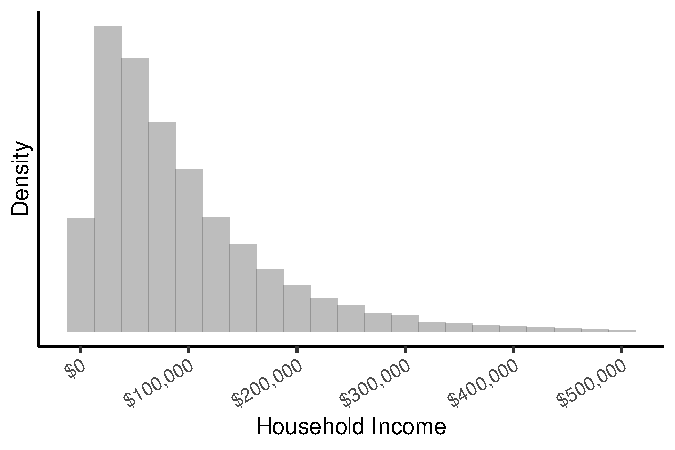
\includegraphics[width = \textwidth]{us2022_hh_dist_big}};
\node<2> at (0,0) {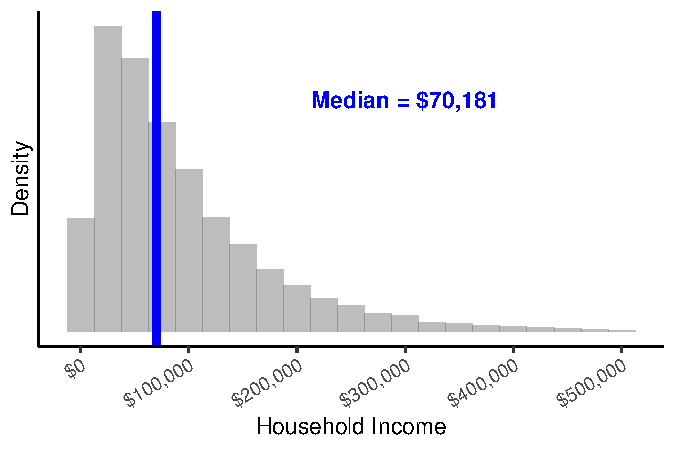
\includegraphics[width = \textwidth]{us2022_hh_dist_median}};
\node<3> at (0,0) {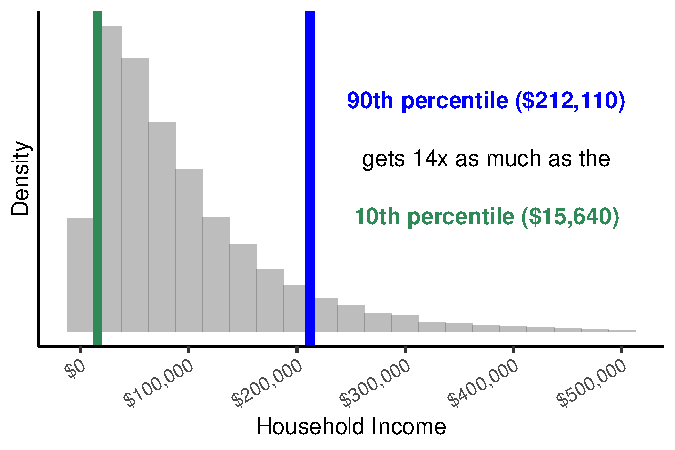
\includegraphics[width = \textwidth]{us2022_hh_dist_9010}};
\end{tikzpicture}

\end{frame}

\begin{frame}
\huge Normative arguments about inequality
\end{frame}

\begin{frame}
\begin{tikzpicture}[x = \textwidth, y = .9\textheight]
\node at (0,0) {};
\node at (1,1) {};
%\node[anchor = north west, font = \large] (title) at (0,1) {\bblue{Studying Social Inequality with Data Science}};
%\node[anchor = north west, font = \footnotesize] (sub) at (title.south west) {Spring 2024. Cornell Info 3370 / 5371.};
\node[anchor = north west] at (0, .93) {\textbf{Activity.} Which income distribution would you prefer? Why?};
\node[font = {\Large\bf}, color = white, fill = black, rounded corners] at (.5, .8) {pollev.com/info3370};
\node[anchor = north west] (a) at (0, .7) {\textbf{Distribution A}};
\node[anchor = north west] (b) at (.5, .7) {\textbf{Distribution B}};
\node[anchor = north west] at (a.south west) {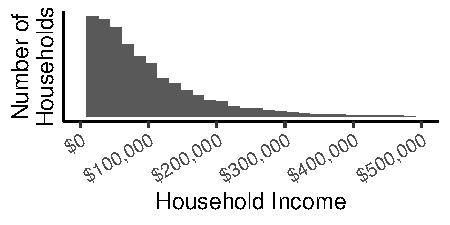
\includegraphics[width= .5\textwidth]{us2022_hh_dist}};
\node[anchor = north west] at (b.south west) {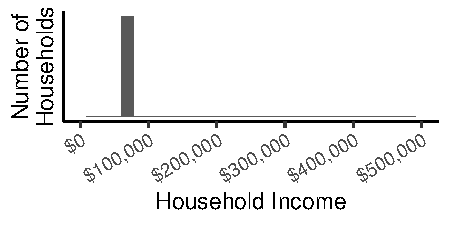
\includegraphics[width= .5\textwidth]{equal_dist}};
\node[anchor = north west, font = \small, align = left] (a1) at (0, .3) {U.S. 2022 distribution};
\node[anchor = north west, font = \small] at (.5, .3) {Everyone gets \$70,181};
\end{tikzpicture}
\end{frame}

\begin{frame}
\begin{tikzpicture}[x = \textwidth, y = \textheight]
\node at (0,0) {};
\node at (1,1) {};
\node[anchor = west] at (0,.5) {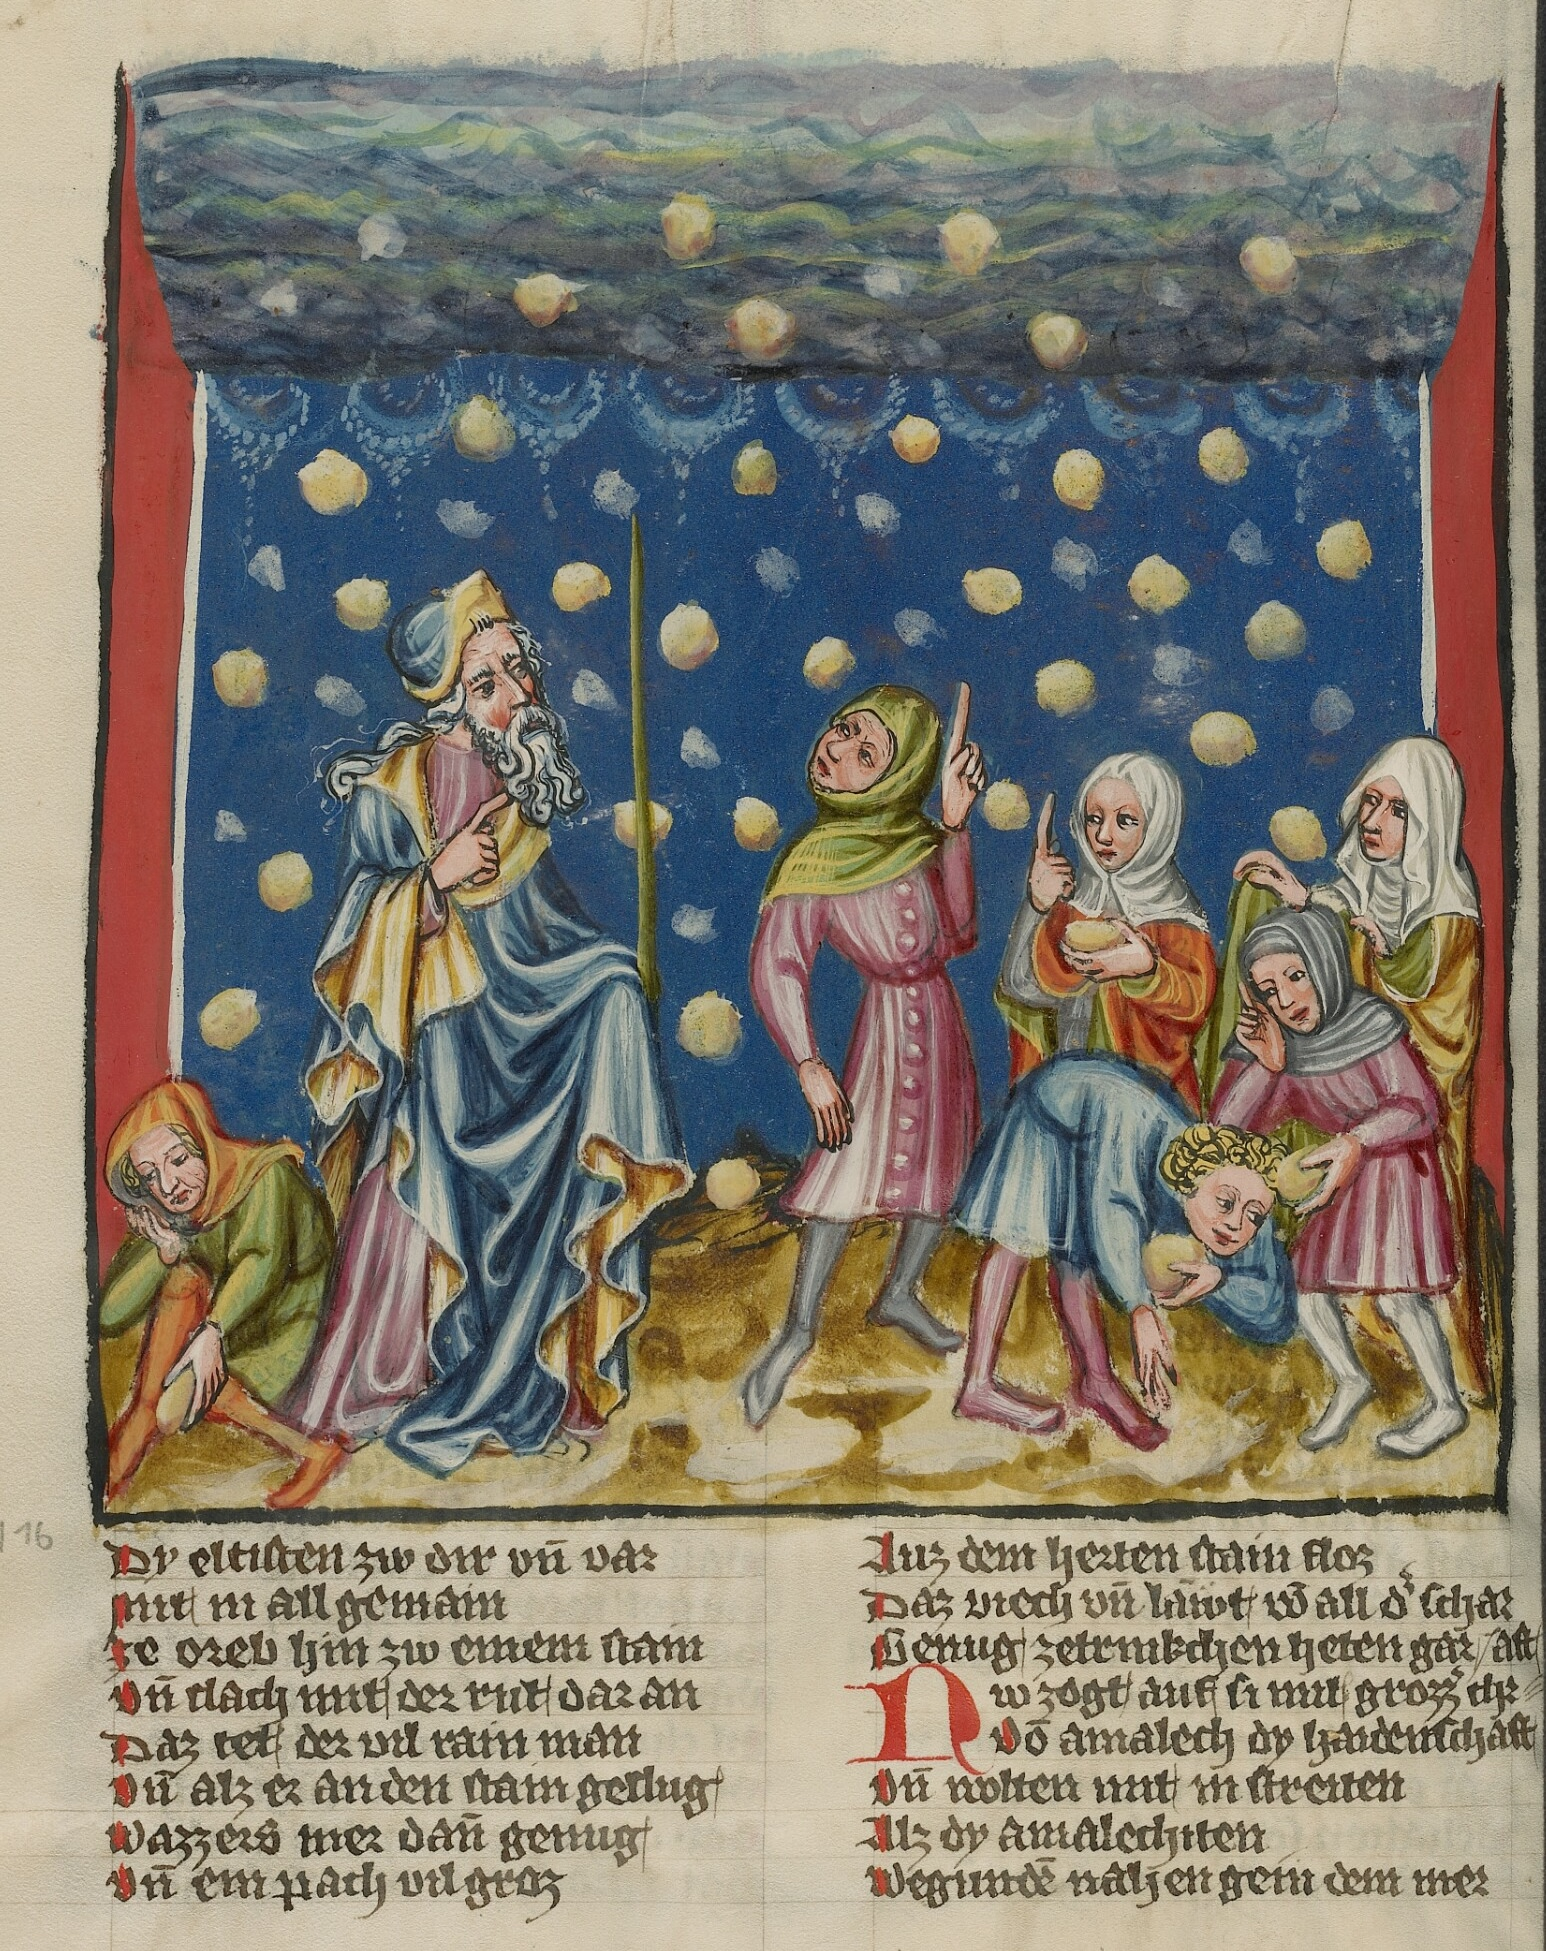
\includegraphics[height = \textheight]{manna}};
\node[anchor = north east, align = right, font = \small] (title) at (1,.4) {The Israelites\\Collecting Manna\\from Heaven};
\node[anchor = north east, align = right, font = \small] (title2) at (title.south east) {Austria\\About 1400--1410};
\node[anchor = north east, align = right, font = \tiny] (title3) at (title2.south east) {Unknown artist\\Getty Open Content Program\\\href{https://www.getty.edu/art/collection/object/105T6R}{getty.edu/art/collection/object/105T6R}};
\node<2->[anchor = north west] (q) at (.62, .95) {Manna drops from heaven};
\node<3->[anchor = north west, align = left] (q2) at (.62,.83) {First pound is more\\helpful than the second};
\node<4->[anchor = north west, align = left] (q3) at (q2.south west) {How should we distribute\\the manna?};
\draw<5-> (q.west) -- (q.east);
\node<5->[anchor = north west] (q) at (.62, .89) {People work for manna};
\end{tikzpicture}
\end{frame}

\begin{frame}

An argument for allowing inequality
\begin{enumerate}
\item unequal rewards motivate work and innovation
\item work and innovation make everyone better off
\end{enumerate}
Thus inequality makes us all better off \vskip .2in \pause
\textbf{Empirical question.} Do unequal places have higher well-being?

\end{frame}

\begin{frame}
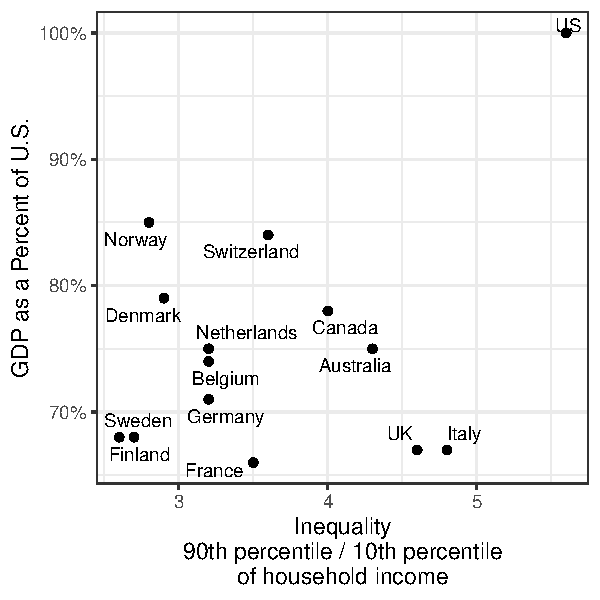
\includegraphics[width = .8\textwidth]{jencks_table1}
\end{frame}
\begin{frame}
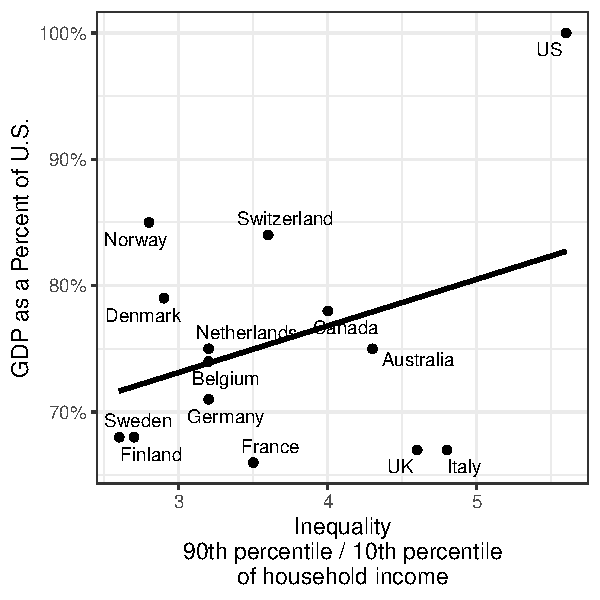
\includegraphics[width = .8\textwidth]{jencks_table1_line}
\end{frame}
\begin{frame}
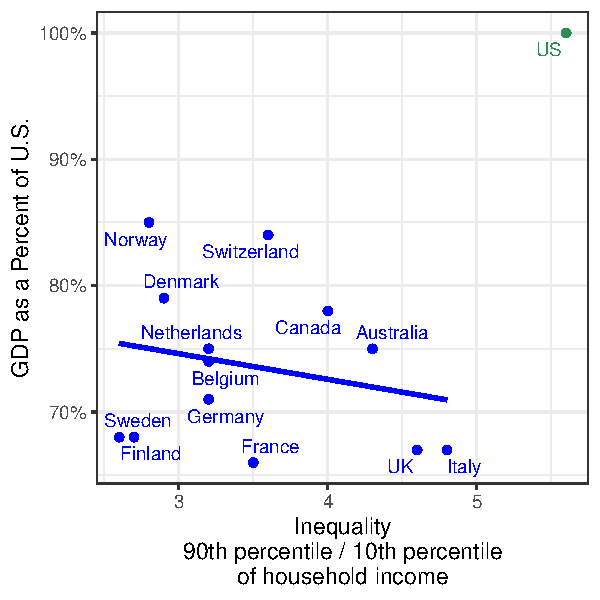
\includegraphics[width = .8\textwidth]{jencks_table1_dropUS}
\end{frame}

\begin{frame}{Goals of the course}

\begin{itemize}
\item visualize economic inequality with graphs\\that summarize survey data
\item connect theories about inequality to\\quantitative empirical evidence
\item evaluate interventions to reduce inequality
\item conduct data analysis using\\the R programming language
\end{itemize}
\end{frame}

\begin{frame}{Plan for the course}

\huge \bref{https://info3370.github.io/}{info3370.github.io}

\end{frame}

\end{document}

\begin{frame}
\begin{huge} A \bblue{normative} question\end{huge} \vskip .2in
What distribution is desirable?
\end{frame}



\begin{frame}
Jencks makes two suppositions (p.~50) \pause
\begin{enumerate}
\item ``manna...dropped from heaven''
\begin{itemize}
\item (no one worked for it)
\end{itemize} \pause
\item ``each additional pound of manna yielded a progressively smaller increase in the recipient's well-being''
\begin{itemize}
\item (diminishing marginal utility)
\end{itemize}
\end{enumerate} \pause \vskip .2in
How should we distribute the manna?
\begin{center}
%To maximize utility,\\we should distribute \bgreen{equally}
\end{center}
\end{frame}

\begin{frame}
\begin{huge} An \bblue{empirical} question\end{huge} \vskip .2in
What distribution do we have?
\end{frame}

\begin{frame}
\begin{tikzpicture}[x = \textwidth, y = .6\textheight]
\node at (0,0) {};
\node at (1,1) {};
\node[anchor = west] at (0,.5) {\includegraphics[height = \textheight]{figures/jencks9010}}; \pause
\node[anchor = south, align = center, font = \footnotesize] at (.7,1.05) {People Sorted\\by Income};
\node[anchor = south, align = center, font = \scriptsize, rotate = 90] at (.65,.5) {Higher income $\rightarrow$};
\foreach \i in {.02,.04,...,.98}{
\node[lightgray, font = \tiny] at (.7,\i) {$\bullet$};
} \pause
\node[blue, font = \tiny] at (.7,.9) {$\bullet$};
\node[anchor = north west, align = center, font = {\scriptsize\bf}, blue] at (.82,.93) {90\%\\earn less};
\draw[->, blue, thick] (.7,.9) -- (.8,.9) -- (.8,.8); \pause
\node[blue, font = \tiny] at (.7,.1) {$\bullet$};
\node[anchor = north west, align = center, font = {\scriptsize\bf}, blue] at (.82,.13) {10\%\\earn less};
\draw[->, blue, thick] (.7,.1) -- (.8,.1) -- (.8,0); \pause
\node[anchor = north, align = center, font = {\scriptsize\bf}, blue] at (.75,-.12) {Summary: $\frac{\text{90th percentile}}{\text{10th percentile}}$};
\end{tikzpicture}
\end{frame}

\end{document}

%\maketitle



\begin{frame}
The following figures are taken from:
\begin{itemize}
\item \bref{https://doi.org/10.1126/science.1251936}{Piketty \& Saez (2014)}
\item \bref{https://www.census.gov/content/dam/Census/library/publications/2022/demo/p60-277.pdf}{U.S. Census Bureau (2022)}
\end{itemize}
\end{frame}

\begin{frame}
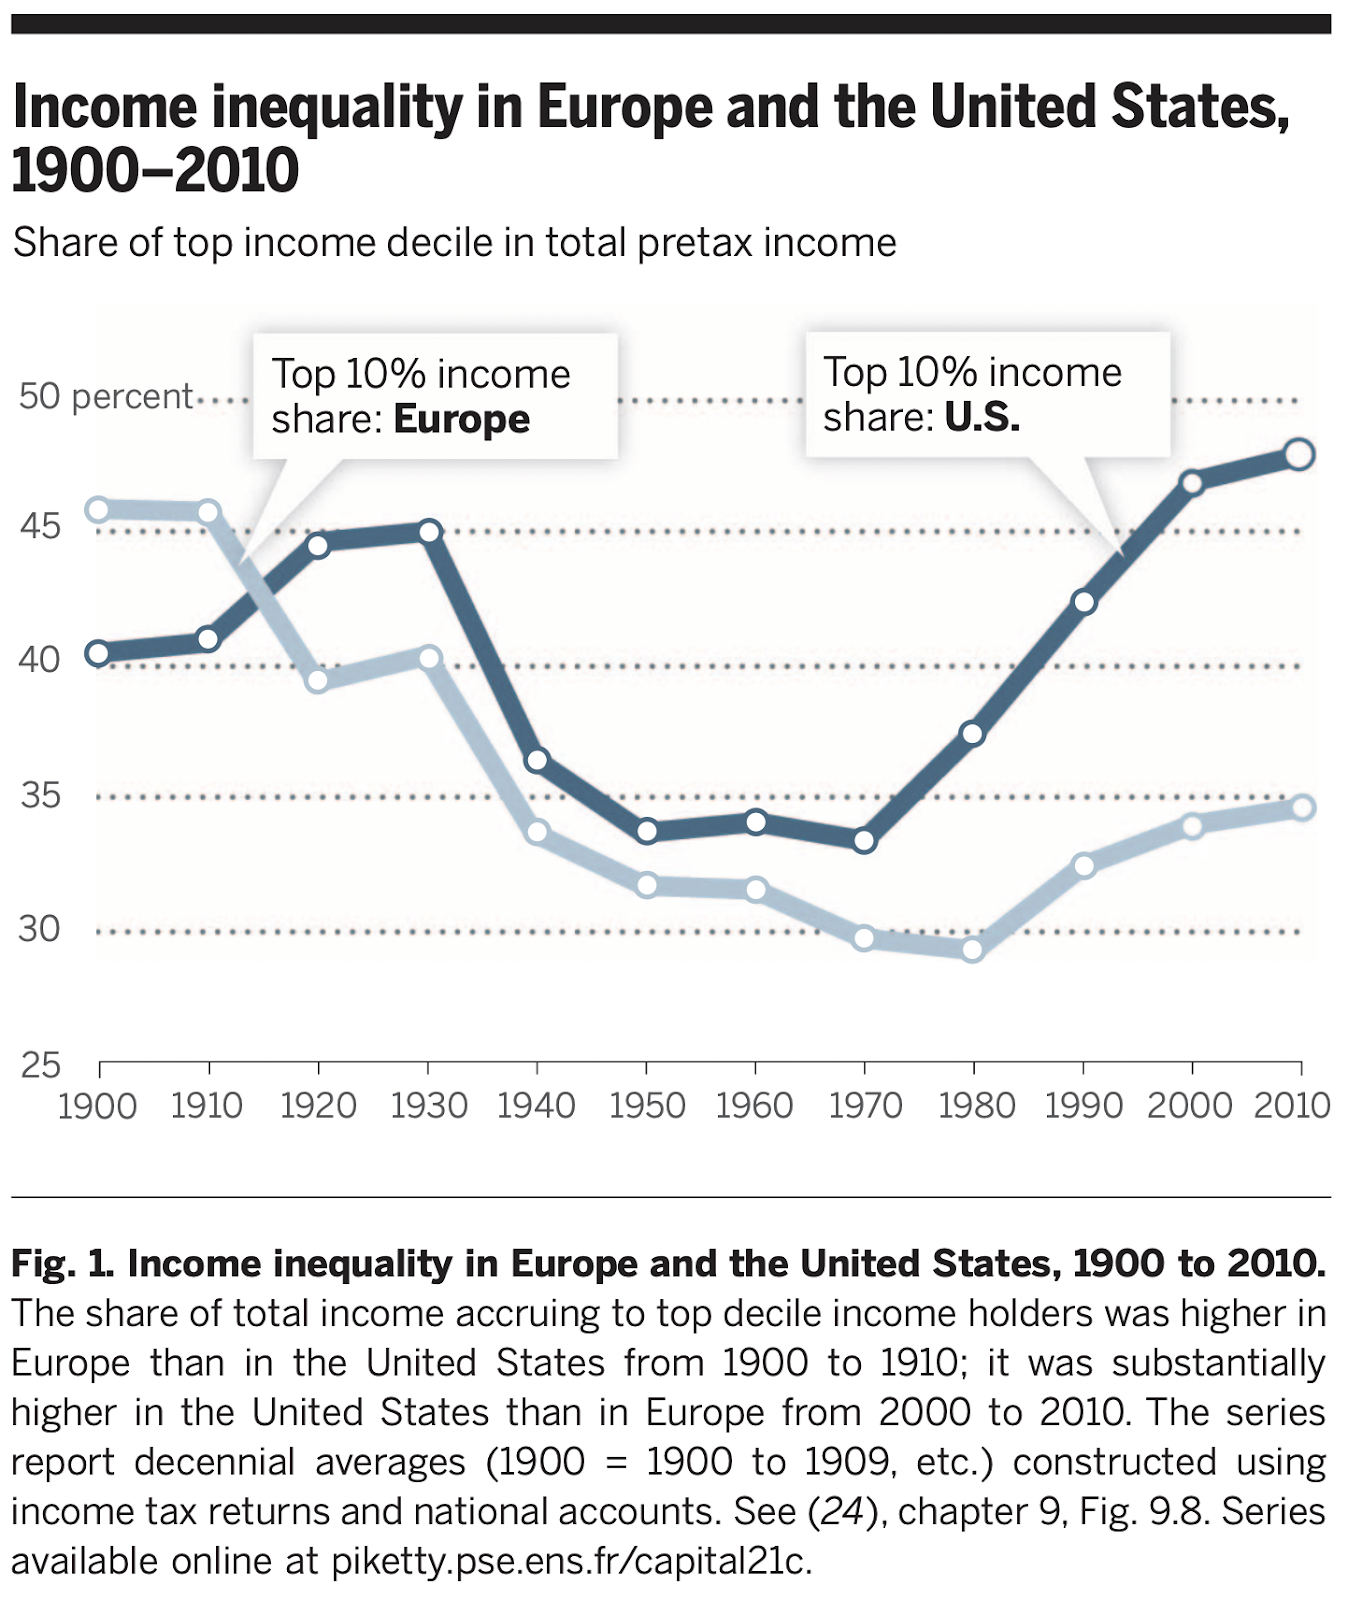
\includegraphics[width = \textwidth]{figures/pikettySaez1.png}
\end{frame}

\begin{frame}
\includegraphics[width = \textwidth]{figures/census1.png}
\end{frame}

\begin{frame}
\begin{tikzpicture}[x = \textwidth, y = \textheight]
\node at (0,0) {};
\node at (1,1) {};
\node[anchor = west] at (0,.5) {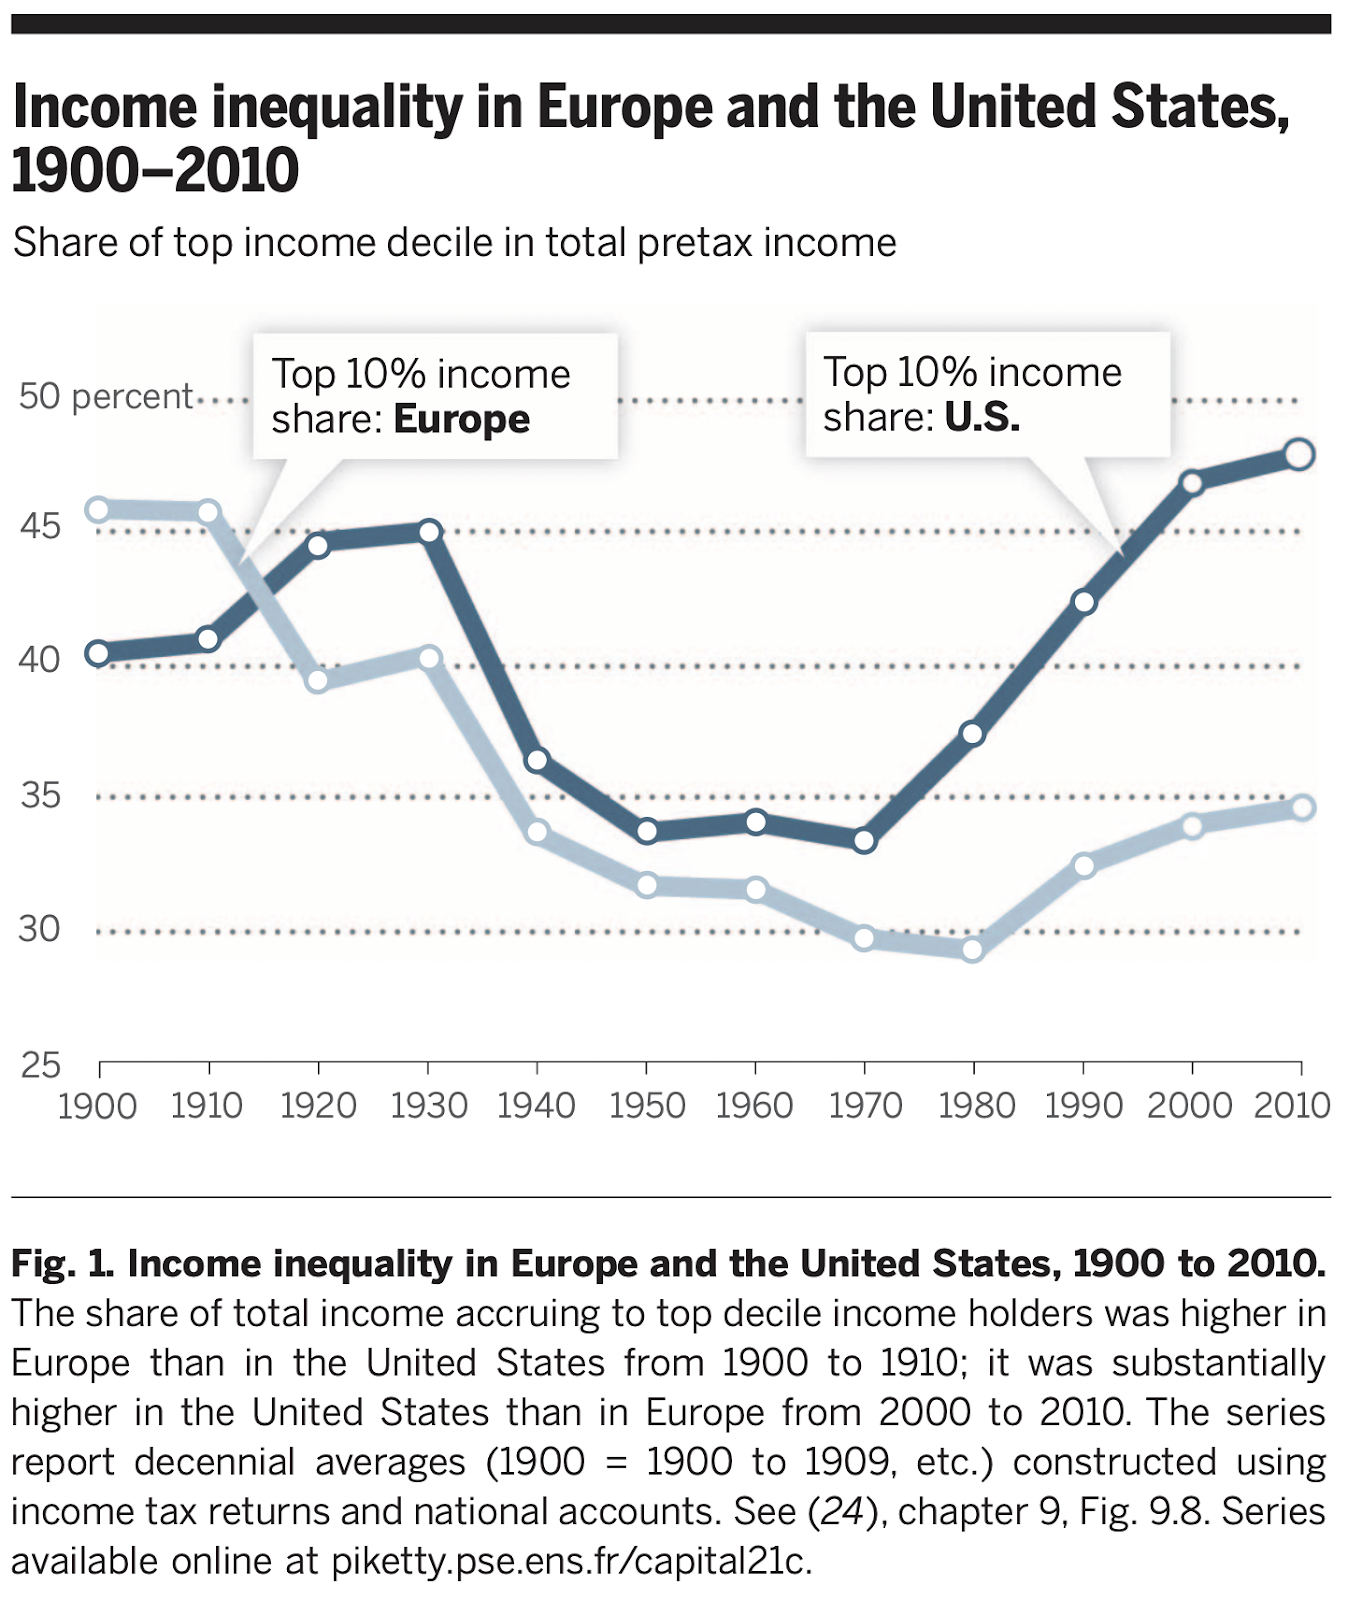
\includegraphics[width = .4\textwidth]{figures/pikettySaez1.png}};
\node[anchor = east] at (1,.5) {\includegraphics[width = .55\textwidth]{figures/census1.png}};
\end{tikzpicture}
\end{frame}

\begin{frame}{Teaching team}
\begin{tikzpicture}[x = \textwidth, y = .9\textheight]
\node at (0,0) {};
\node at (1,1) {};
\node[anchor = north, align = center] at (.25,.7) {Ian Lundberg};
\node[anchor = north, align = center] at (.75,.7) {Federica Bologna};
\node[anchor = north, align = center] at (.1,.3) {Abby\\Sachar};
\node[anchor = north, align = center] at (.3,.3) {Amaan\\Rehan};
\node[anchor = north, align = center] at (.5,.3) {Chase\\Young};
\node[anchor = north, align = center] at (.7,.3) {Elizabeth\\Moon};
\node[anchor = north, align = center] at (.9,.3) {Shirley\\Zhang};
\node[anchor = south] at (.25,.7) {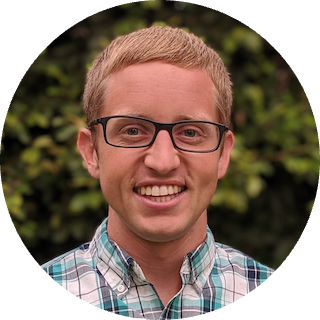
\includegraphics[height = .2\textheight]{figures/ian}};
\node[anchor = south] at (.75,.7) {\includegraphics[height = .2\textheight]{figures/fede}};
\node[anchor = south] at (.1,.3) {\includegraphics[height = .2\textheight]{figures/abby}};
\node[anchor = south] at (.3,.3) {\includegraphics[height = .2\textheight]{figures/amaan}};
\node[anchor = south] at (.5,.3) {\includegraphics[height = .2\textheight]{figures/chase}};
\node[anchor = south] at (.7,.3) {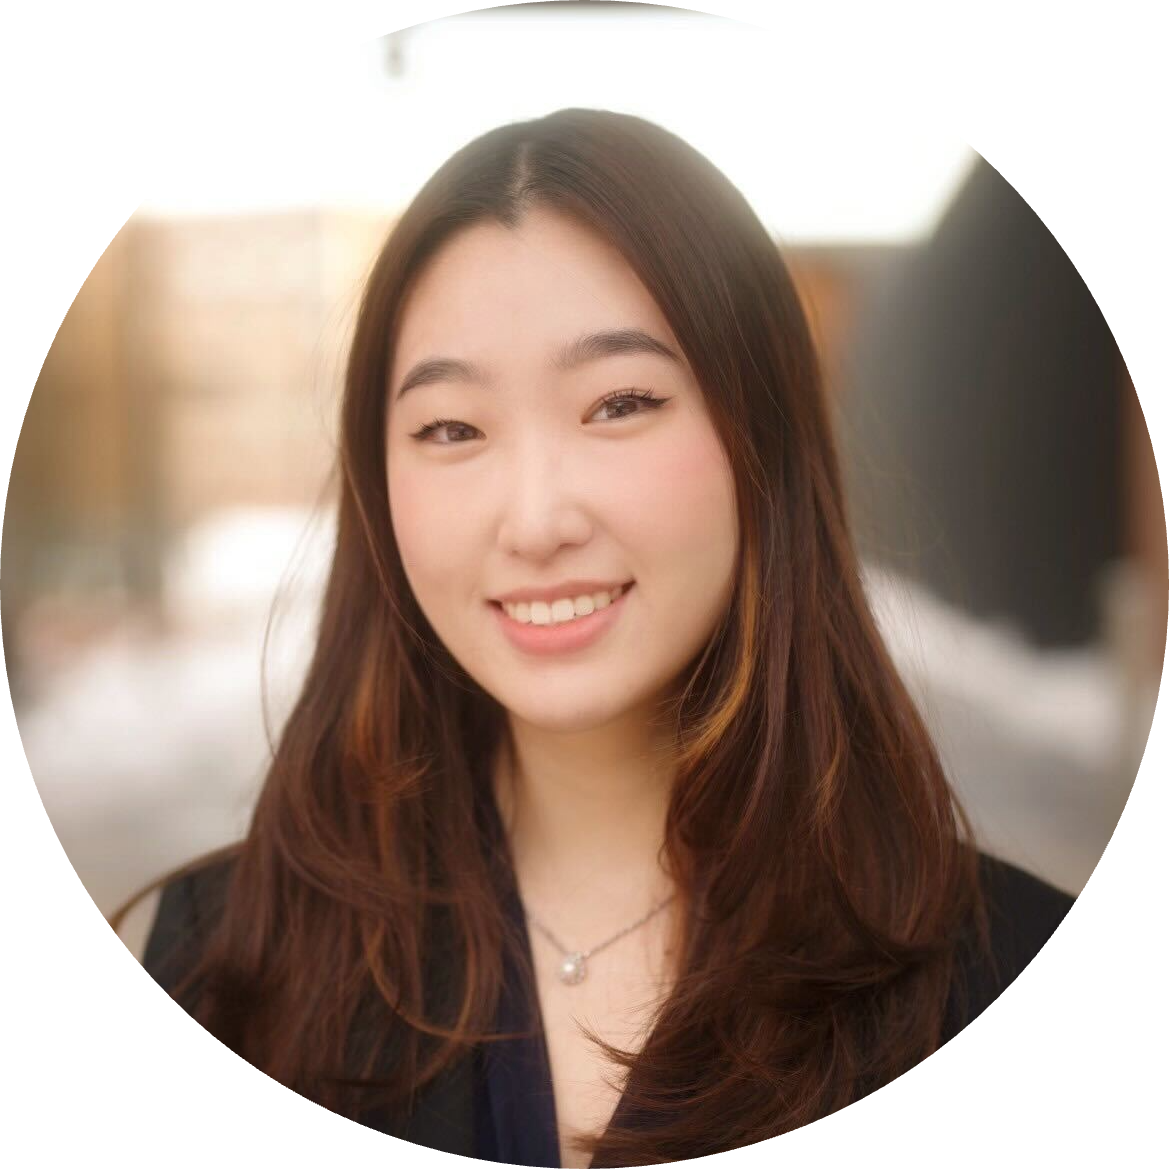
\includegraphics[height = .2\textheight]{figures/liz}};
\node[anchor = south] at (.9,.3) {\includegraphics[height = .2\textheight]{figures/shirley}};
\end{tikzpicture}
\end{frame}



\begin{frame}
\begin{tikzpicture}[x = \textwidth, y = \textheight]
\node at (0,0) {};
\node at (1,1) {};
\node[anchor = north west, align = left, font = \huge] at (0,.9) {Studying\\Social Inequality\\with Data Science};
\node[anchor = north east, align = right] (number) at (1,.9) {INFO 3370 / 5371\\Spring 2023};
\node[anchor = north east, font = \Large, align = right] at (1,.7) {\bblue{2. Does inequality}\\\bblue{matter?}};
\node[anchor = north west] at (0,.55) {\includegraphics[width = \textwidth]{figures/jencks1}};
\end{tikzpicture}
\end{frame}

\goalsframe

\begin{frame}
\centering
\begin{tikzpicture}
\node at (-6,0) {};
\node[anchor = south] at (0,0) {\includegraphics[width = .8\textwidth, trim = {0 7.3in 0 0}, clip]{figures/jencks3}};
\node[anchor = north] at (0,0) {\includegraphics[width = .8\textwidth, trim = {0 0 0 9.8in}, clip]{figures/jencks3}};
% Block Canada
\draw<1-2>[fill = white, draw = white] (-2.5,-.6) rectangle (4,.3);
% Block Australia
\draw[fill = white, draw = white] (-2.5,-1.6) rectangle (4,-1);
\node<2>[align = left, anchor = north west] at (-6, 0) {\bblue{Question:}\\Where would\\you rather live:\\U.K. or U.S.?};
\node<4>[align = left, anchor = north west] at (-6, 0) {\bblue{Question:}\\Where would\\you rather live:\\Canada or U.S.?};
\node<5>[align = left, anchor = north west] at (-6,3) {What part is\\\bgreen{empirical}\\and what part is\\\bgreen{normative}?};
\end{tikzpicture}
\end{frame}



\begin{frame}
\begin{huge}Recognize \bblue{cultural views}\end{huge}\vskip .2in
that conflict with facts
\end{frame}

%\begin{frame}{Why is inequality so high in the U.S.?}

%``The United States is unusually unequal partly because it makes little effort to limit wage inequality: the minimum wage is low, and American law makes unionization relatively difficult. In addition, the United States transfers less money to those who are not working than most other rich democracies.'' \vskip .1in

%--- Jencks p. 53

%\end{frame}

\begin{frame}
\begin{tikzpicture}[x = \textwidth]
\node[anchor = west] at (0,0) {\includegraphics[height = .8\textheight]{figures/declaration}};
\node[anchor = east, align = right] at (1,0) {We hold these truths\\to be self-evident,\\that all men are\\created equal...};
\end{tikzpicture}
\end{frame}

\begin{frame}
\begin{tikzpicture}[x = \textwidth]
\node at (0,0) {};
\node at (1,1) {};
\node[anchor = west] (picture) at (0,0) {\includegraphics[height = .6\textheight]{figures/detoc}};
\node[anchor = north west, font = \tiny, align = left] at (picture.south west) {\textbf{Alexis de Tocqueville}\\By Théodore Chassériau, 1850\\Public domain, via \href{https://commons.wikimedia.org/wiki/File:Alexis_de_tocqueville.jpg}{Wikimedia Commons}}; \pause
\node[anchor = east, align = left, text width = .5\textwidth] (quote) at (1,0) {\raggedright Democratic communities...call for equality in freedom; and if they cannot obtain that, they still call for equality in slavery. They will endure poverty, servitude, barbarism, but they will not endure aristocracy. \vskip .05in };
\node[anchor = north west, font = \footnotesize, align = left] at (quote.south west) {1840, \href{https://xroads.virginia.edu/~Hyper/DETOC/ch2_01.htm}{Influence of Democracy on the}\\\href{https://xroads.virginia.edu/~Hyper/DETOC/ch2_01.htm}{Feelings of the Americans}};
\end{tikzpicture}
\end{frame}

\begin{frame}

American politicians present themselves to the public as being just like everyone else, and once they step outside their offices, Americans all wear jeans. \vskip .2in

--- Jencks p.~53 \vskip .4in

\begin{center}
\includegraphics[width = .3\textwidth]{figures/levis}\\
\begin{tiny}Source: \href{https://commons.wikimedia.org/wiki/File:Levis_logo_1892.png}{Wikimedia}\end{tiny}
\end{center}

\end{frame}

\goalsframe

\begin{frame}{Before next class: Install R}

\bref{https://info3370.github.io/lessonplans/1c/}{info3370.github.io/lessonplans/1c/}

\end{frame}

\end{document}

